\section{Interface}

Nesta seção serão descritos os elementos da interação entre o jogador e o
jogo.

\subsection{HUD}

A tela do jogador terá as informações a seguir, seguindo o modelo da
Figura \ref{fig:hud}
\begin{figure}[!ht]
 \centering
 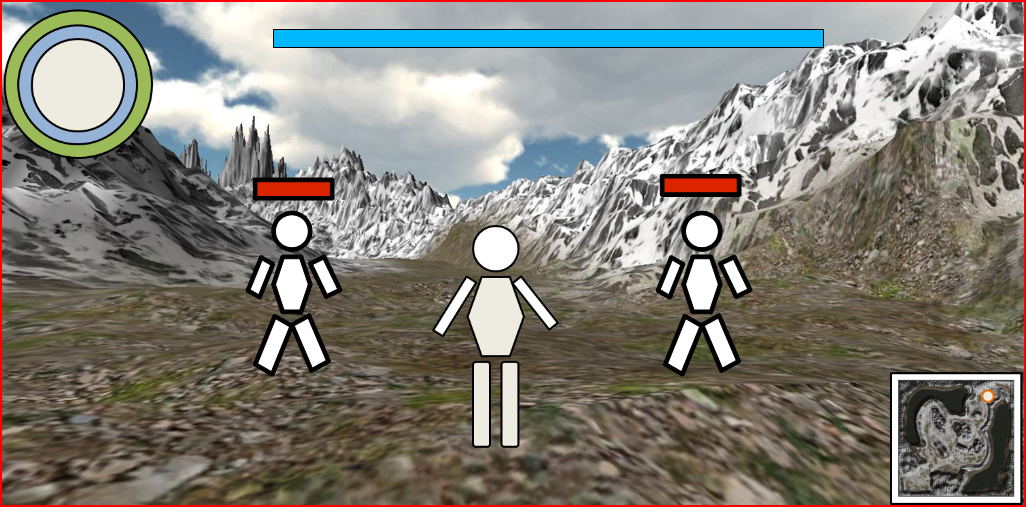
\includegraphics[scale=0.59]{hud.png}
 \caption{HUD}
 \label{fig:hud}
\end{figure}
\begin{enumerate}
 \item {\bf Marcador de vida:} Canto superior esquerdo da tela, no 
formato de uma faixa circular. Na figura está demonstrado pela faixa
verde;
 \item {\bf Marcador de energia/temperatura:} Quando houver este marcador,
ele estará no canto superior esquerdo da tela, também no formato
de uma faixa circular, dentro da faixa do marcador de vida. Na primeira
fase será o marcador de energia e, na segunda, o de temperatura. Não
existirá este marcador na terceira fase. Na figura está indicado pela 
faixa azul dentro da faixa verde;
 \item {\bf Minimapa:} Canto inferior direito, em forma de quadrado.
Será fixo e semi-transparente. Mostrará um esboço do mapa e um triângulo
indicando a posição e direção de Medrash. Existirá nas 3 fases;
 \item {\bf Barra de vida dos inimigos:} Ficará sobre a cabeça do inimigo,
indicando quantos pontos de vida ele ainda possui. Indicado na figura
como barras vermelhas;
 \item {\bf Barra de tempo:} Esta barra indicará indicará o tempo restante
 para completar a batalha final. Portanto, existe apenas na fase 3.
Seu tamanho irá diminuir progressivamente, indicando o tempo se esgotando. Na 
figura, a barra azul no topo da tela indica a Barra de Tempo.
\end{enumerate}

\subsection{Menus}

O jogo terá três menus. Um deles será o menu principal do jogo, o 
outro será o menu de pausa e o último será um menu entre fases.

\subsubsection{Menu Principal}

O menu principal terá as seguintes opções:
\begin{itemize}
 \item {\bf Começar novo jogo:} Apaga todas informações sobre o jogo atual
se houver e inicia um novo jogo;
 \item {\bf Continuar jogo:} Se houver um jogo em progresso, permite que
o usuário continue o mesmo. Caso contrário, esta opção estará desativada;
 \item {\bf Carregar jogo:} Permite que o usuário carregue algum jogo
gravado, se houver;
 \item {\bf Sair do jogo:} Sai do jogo, finalizando o software.
\end{itemize}

\subsubsection{Menu de Pausa}
O menu de pausa só pode ser acessado durante o jogo e contém as seguintes
opções:
\begin{itemize}
 \item {\bf Continuar o jogo:} Sai do menu de pausa;
 \item {\bf Voltar ao menu principal:} Sai do jogo e volta ao menu 
principal. Não salva o jogo;
 \item {\bf Sair do jogo:} Sai do jogo e finaliza o software.
\end{itemize}

\subsection{Menu entre fases}
Ao final das fases 1 e 2 será exibido um menu que irá mostrar a pontuação do
personagem, assim como as opções:
\begin{itemize}
 \item {\bf Salvar jogo:} Permite que o jogador salve o progresso;
 \item {\bf Próxima fase:} Continua para a próxima fase;
 \item {\bf Voltar ao menu principal:} Sai do jogo e volta ao menu principal;
 \item {\bf Sair do jogo:} Sai do jogo e finaliza o software.
\end{itemize}
